\chapter{Introduction}
\label{ch:intro}

\section{Motivation}

State-of-the-art (SOTA) object classification methods rely on deep learning models that are either trained end-to-end on the target application or initially trained on one task and subsequently fine-tuned for a different one. In both cases the resulting models are \emph{monolithic}: a single network is trained on a large dataset and performs feature extraction and classification jointly. Such models are highly effective when the set of object classes is fixed and known at training or fine-tuning time. When new object classes must be incorporated, however, the entire model must be retrained or fine-tuned. This procedure requires significant computational resources, demands access to the original training dataset and, in many cases, leads to \emph{catastrophic forgetting} of previously learned classes \cite{catastrophic}.

A natural way to integrate new classes while avoiding catastrophic forgetting is to formulate the problem as continual or class-incremental classification, in which the algorithm must learn to distinguish an ever-growing number of categories \cite{vandeVen}. In this paradigm, a \emph{task} corresponds to a distinct portion of the training experience, presented sequentially to the model. Instead of having access to the entire dataset at once, as in conventional supervised learning, the model receives data in sequential chunks \cite{taskarithmeticloracontinual}. Each task typically corresponds to a set of new classes that must be recognised. The central challenge is that when the model is updated task by task, it tends to overwrite previously acquired knowledge: monolithic models are structurally ill-suited for this scenario, and an alternative paradigm is therefore required.

This limitation has motivated the SOTA in continual classification to focus on balancing \emph{stability} and \emph{plasticity}. Stability refers to a model's ability to preserve previously learned knowledge; plasticity describes its capacity to adapt and incorporate new tasks \cite{API}. Traditional approaches rarely optimise both properties simultaneously: when stability dominates, the model struggles to integrate new knowledge; when plasticity dominates, it loses access to past information. This trade-off is compounded by the limited capacity of neural networks to integrate new representations without interfering with old ones and by the need to continually adjust the network's structure to match the growing number of object classes. The dominant view in the literature therefore treats continual learning as a problem of \emph{parameter interference}: learning new classes requires updating network weights, which may overwrite previously acquired knowledge, and most existing methods attempt to control this process through regularization, rehearsal buffers, or architectural adaptations \cite{CL}. Although effective, these strategies share a common premise that this thesis sets out to challenge: that incremental learning must be achieved through continuous, careful optimization of the parameters of the network responsible for feature extraction.

This premise diverges significantly from the organisational principles of biological vision. The human visual system relies on early cortical regions responsible for feature extraction that mature and stabilize during the initial postnatal weeks or months~\cite{Sluyters90}, providing highly stable feature representations that remain stationary throughout adulthood. However, despite this invariant sensory foundation, human lifelong learning persists. Higher-order cognitive systems seamlessly map these fixed perceptual representations onto newly encountered semantic categories, even if acquiring knowledge of a new object class can occasionally result in a slight, localized reduction in the ability to distinguish highly similar classes over time.

 
A directly analogous structural separation has recently become achievable in computer vision through large-scale visual foundation models. By leveraging pre-trained foundation models such as DINOv2 \cite{oquab2024dinov}—which are trained on massive, diverse datasets—downstream systems obtain highly discriminative representations that remain completely stable once frozen. In this stationary feature space, \emph{representation drift}—the gradual shifting of a network's internal features during sequential task updates, which serves as the primary driver of catastrophic forgetting—is eliminated by construction: the coordinates describing each class no longer change when a new task arrives. Mirroring the biological paradigm, class-incremental learning can thus be conceptually reframed: rather than protecting network parameters from destructive interference, the challenge becomes one of accurately modeling the distribution of new classes within a robust, fixed embedding space. This perspective motivates the present work: once a sufficiently discriminative and stable feature space is secured, the core challenge of continual learning shifts from \emph{preventing forgetting} to \emph{estimating probability densities}.

Building on this observation, this thesis proposes a continual-learning object-recognition system organized into two complementary, decoupled components. As illustrated in Figure~\ref{fig:intro_overview}, the first component is a \emph{feature extractor} derived from a frozen, pre-trained foundation model. This encoder maps an input image to a static, highly discriminative feature vector $\vec{x}$ in a shared embedding space. Crucially, these representations must be sufficiently general to characterize arbitrary object classes, including those unseen during the foundation model's pre-training. The second component is a \emph{statistical classifier} composed of a collection of independent, class-conditional Gaussian models ($G_1, \dots, G_N$). When a new class arrives, a corresponding Gaussian model is estimated and integrated without altering or accessing previously learned class models. At inference time, classification is performed by computing the posterior probability $p(c_k \vert{} \vec{x})$ for each class and assigning the input to the class that yields the maximum value, in direct analogy to a generative Bayes classifier. This modular, two-stage framework is developed in full mathematical detail in Chapter~\ref{methodology}.

\begin{figure}[htb]
	\centering
	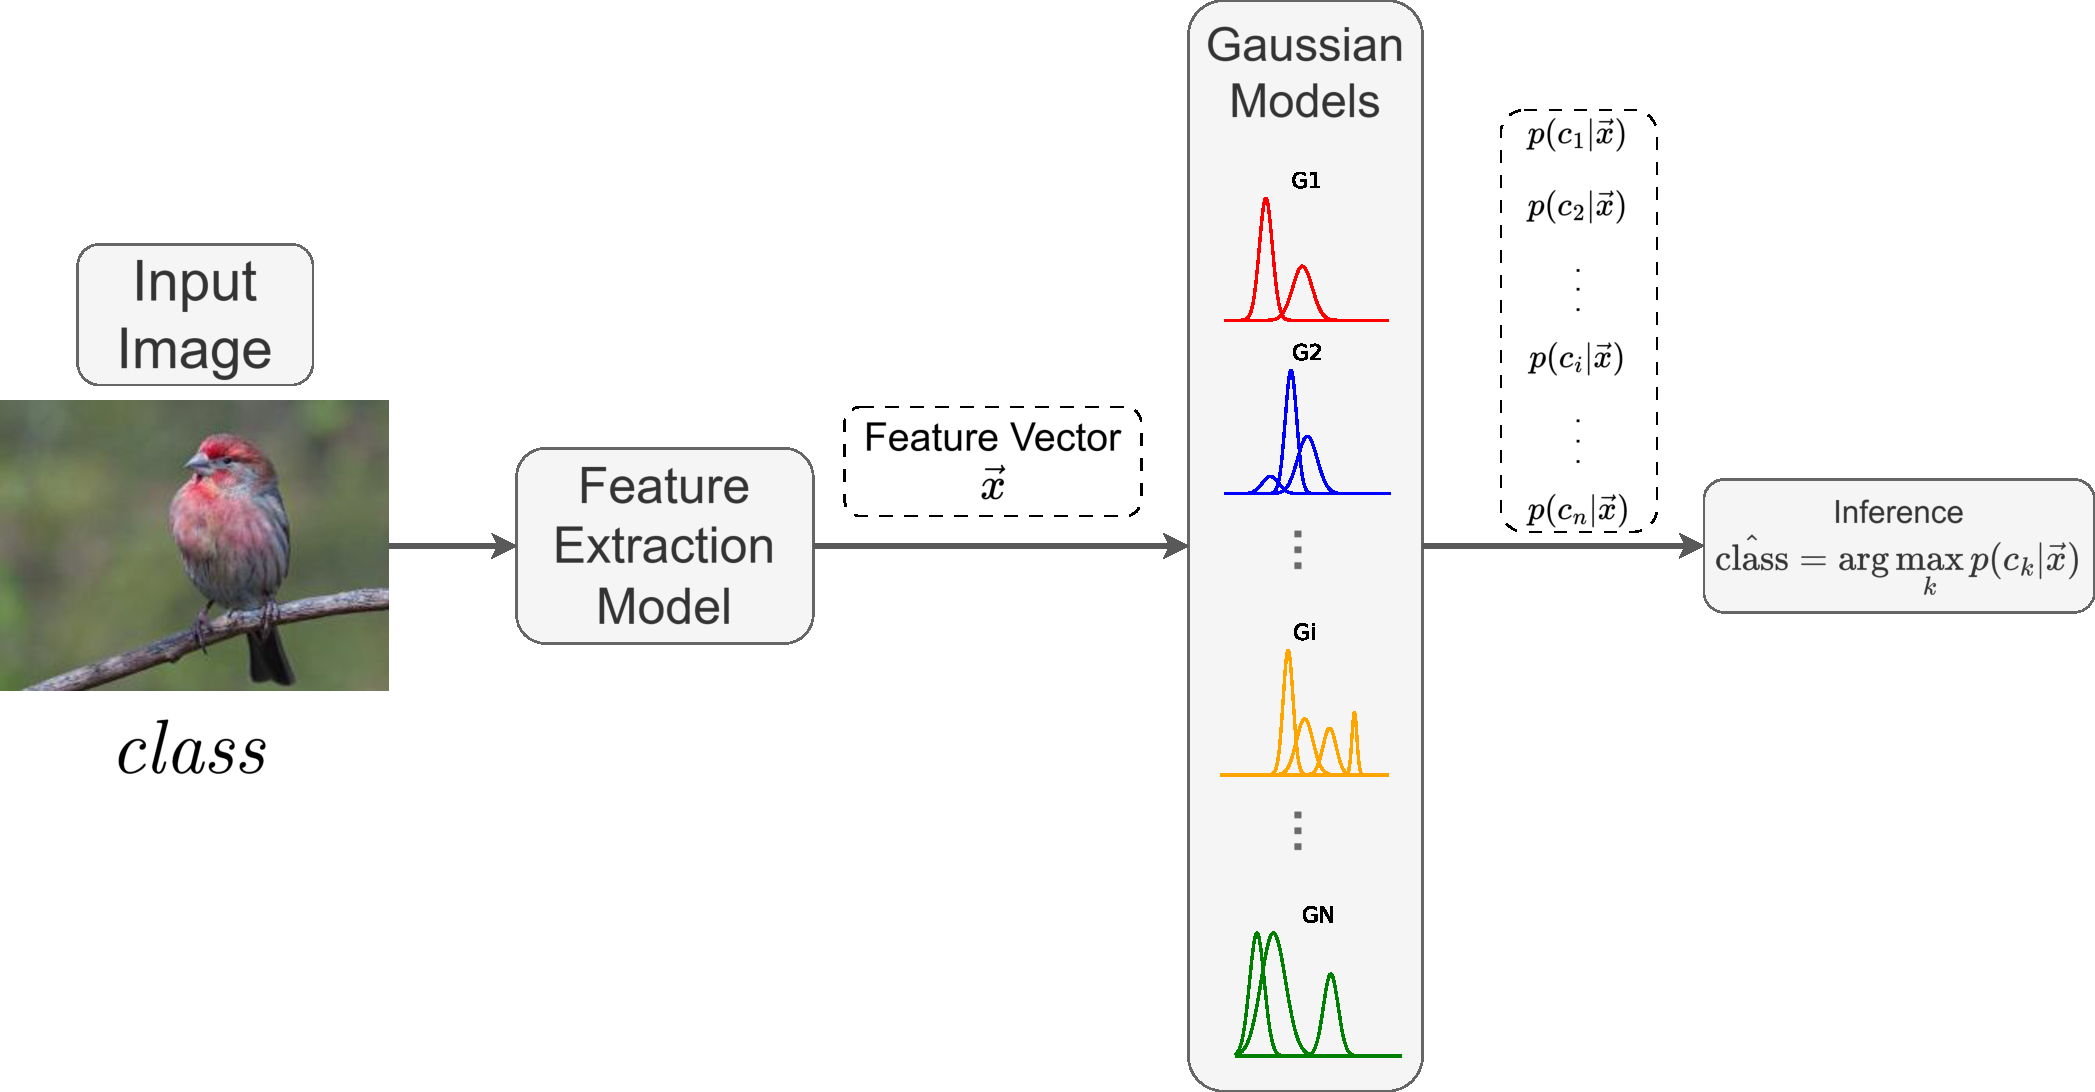
\includegraphics[width=0.7\textwidth]{imagenes/methodology/block_diagram_approach.pdf}
	\caption{Overview of the continual-learning framework: a frozen foundation model extracts features $\vec{x}$, classes are modeled independently as Gaussians ($G_k$) to allow dynamic registration without retraining, and inference predicts via Bayesian posterior maximization.}
	\label{fig:intro_overview}
\end{figure}

Gaussian class representations offer two key advantages that make them particularly well suited to this reframed problem. First, each class is modelled independently from the rest, so incorporating a new class amounts to estimating a small number of sufficient statistics (mean and covariance) and does not require any modification of the previously stored class models; this yields incremental updates that are exact and gradient-free, and that produce zero catastrophic forgetting by construction. Second, Gaussian models are compact: they encode each class in a few parameters that can be estimated from a modest sample budget and refined as new samples become available, without any storage of the underlying images. This second property, however, is far from trivial in practice: because the dimensionality $d$ of foundation-model embeddings (typically in the hundreds) is frequently comparable to, or larger than, the number of training samples $n_c$ available per class, the empirical covariance matrix is structurally rank-deficient whenever $n_c < d$. This thesis studies this small-sample regime in detail, evaluating a full spectrum of covariance parameterisations---from diagonal to full covariance matrices, including shared and shrinkage-based estimators.

Because the entire framework rests on the assumption that class-conditional features are approximately Gaussian, this assumption cannot be taken for granted: it must be empirically validated rather than merely postulated. This thesis therefore complements its architectural proposal with a rigorous statistical characterisation of the DINOv2 embedding space, combining moment-based diagnostics (skewness and excess kurtosis) with formal hypothesis tests---the D'Agostino--Pearson omnibus test \cite{dagostino1971omnibus,dagostino1973tests} for univariate normality and a diagonal adaptation of the Henze--Zirkler test \cite{henze1990class} for multivariate normality under severe rank deficiency. In parallel, the \emph{Bhattacharyya distance} is used to quantify inter-class separability and to establish a principled theoretical ceiling on the accuracy that any Gaussian classifier can achieve in a given feature space. This separability analysis is not merely descriptive: it is used throughout this thesis to identify, explain, and visualise the specific pairs of classes whose overlapping Gaussian distributions constitute the dominant source of classification error observed in this framework, as opposed to any degradation of previously learned representations.

\section{Hypothesis}

We hypothesize that the combination of an independent class-conditional Gaussian model and a frozen pre-trained feature extractor provides a robust framework for continual object classification. By enabling the addition of new classes without full-model retraining, this design eliminates catastrophic forgetting while maintaining a simple, compact architecture.

\section{General Objective}

The main objective of this thesis is to develop and to validate a continual learning framework for object classification using pre-trained foundation models and independent class-conditional Gaussian models as classifiers, with the purpose of enabling the incremental incorporation of new classes while preventing catastrophic forgetting.

\section{Specific Objectives}

For the purpose of fulfilling the general objective and verifying the hypothesis of this work, the following specific objectives are defined:

\begin{itemize}

	\item To assess the practical performance of the proposed framework across its own architectural variations—including different covariance-matrix estimators and Mixture-of-Gaussian variants—as well as against state-of-the-art baselines.
	
	\item To conduct an in-depth empirical analysis of the system's performance, measuring the effect of upstream backbone representations, progressive class expansion, confidence calibration metrics, and downstream computational cost.
	
	\item To statistically validate the underlying assumptions of the framework by analyzing the datasets representations within the feature extractor embedding space, specifically assessing the Gaussianity of class-conditional feature distributions, evaluating their spectral structure, and quantifying inter-class separability to identify the sources of residual classification error.

\end{itemize}

\section{Contributions}

The principal contributions of this thesis are the following:
\begin{enumerate}
	\item A gradient-free class-incremental learning framework that pairs a frozen DINOv2 backbone with independent, closed-form class-conditional Gaussian models, eliminating catastrophic forgetting by construction rather than by mitigation, together with a systematic evaluation of five covariance parameterisations (diagonal, full, hybrid, shared, and shrinkage-based) and their mixture-of-Gaussian extensions.
	\item A rigorous, multi-layered statistical validation of the Gaussianity assumption underlying the framework---combining moment-based diagnostics, the D'Agostino--Pearson omnibus test, and a diagonal adaptation of the Henze--Zirkler test for both univariate and multivariate normality under severe rank deficiency---that had not previously been carried out for foundation-model embedding spaces at this level of detail.
	\item A quantitative link between inter-class separability, measured via the pairwise Bhattacharyya distance, and the specific, named class pairs that account for the residual classification error of the proposed classifier, reframing that error as a property of the embedding space rather than of the classifier itself.
\end{enumerate}

\section{Thesis Structure}

The remainder of the document is organised as follows.

\paragraph{Chapter~\ref{ch:framework} -- Continual Learning and Foundation Models.} Covers the background needed to situate this work: the basics of artificial intelligence, machine learning, and deep learning applied to object classification, then continual learning itself, including catastrophic forgetting, the stability--plasticity dilemma, and the main families of existing solutions (rehearsal-, regularisation-, architecture-, and prompt-based methods, plus the classifier-adaptation and class-prototype approaches closest to what is proposed here). It closes with the Vision Transformer and the DINOv2 backbone used throughout this thesis.

\paragraph{Chapter~\ref{ch:gaussian_space} -- Statistical and Probabilistic Foundations of the Feature Space.} Lays out the mathematical and statistical tools the framework depends on: Bayesian classification and the Maximum A Posteriori rule, the Mixture-of-Gaussians model, and covariance estimation in the high-dimensional, small-sample regime typical of foundation-model embeddings. It also introduces the spectral tools used to describe the intrinsic dimensionality of the feature space, the tests used later to check the Gaussianity assumption, the Bhattacharyya and Euclidean separability metrics, and the confidence and calibration metrics used to judge how trustworthy the predictions are.

\paragraph{Chapter~\ref{methodology} -- Modelling Class Densities in a Frozen Feature Space.} Presents the proposed architecture in detail: a frozen encoder paired with independent, class-conditional Gaussian models updated in closed form, followed by the full family of covariance estimators evaluated in this thesis (diagonal, full, hybrid, OAS, Ledoit-Wolf, and shared covariance) and their Mixture-of-Gaussians extensions.

\paragraph{Chapter~\ref{ch:results} -- Experimental Results and Analysis.} Reports the experimental protocols and the resulting analysis: the datasets and evaluation protocol, calibration and covariance-estimator performance across benchmarks, accuracy as classes are added incrementally, inter-class separability and the specific class pairs behind the residual error, sensitivity to the choice of backbone, the spectral structure of the DINOv2 embedding space, and the empirical validation of the Gaussianity assumption. Across every one of these analyses, MOG4-Shared is evaluated alongside the rest of the estimators and identified as the strongest overall configuration once accuracy, calibration, and computational cost are all taken into account.

\paragraph{Chapter~\ref{ch:conclusion} -- Conclusion.} Draws together the central findings of the thesis, discusses the limitations of the current framework, and outlines directions for future work that follow directly from those limitations.
